\section{实验室催化反应器}


\begin{frame}
    \frametitle{实验室催化反应器}

    实验室用的催化反应器的共同特点：
    \begin{itemize}
        \item 规模小
        \item 催化剂用量少
    \end{itemize}

    \bigskip
    多相催化反应动力学研究的目的：
    \begin{itemize}
        \item 测得不同温度、压力和反应物系组成等条件下的反应速率数据，再将众多的反应速率数据与其有关的影响因素相关联，整理出反应速率方程。
    \end{itemize}
    \bigskip
    影响反应速率的主要因素：
    \begin{itemize}
        \item 温度
        \item 反应物系的组成
    \end{itemize}

\end{frame}



\begin{frame}
    \frametitle{实验室催化反应器}

    浓度梯度和温度梯度的消除：
    \begin{itemize}
        \item 催化剂粒度越小，有效因子越大，有效因子等于1时，颗粒内就不存在浓度和温度梯度。
        \item 再用此粒度的催化剂改变反应气体的质量速度做实验，以确定相间梯度不存在时的最小质量速度。
        \item 反应器内的轴向和径向梯度与$d_t/d_p$，$L_r/d_p$以及流体力学条件和反应物系的物理性质有关。简单地说是与反应器内气体的流动型式有关。
    \end{itemize}
    \bigskip
    实验室催化反应器两点最基本的要求是：
    \begin{enumerate}
        \item 等温操作；
        \item 反应气体保持理想流型。
    \end{enumerate}

\end{frame}



\begin{frame}
    \frametitle{实验室催化反应器}

    实验室中用以进行动力学研究的催化反应器主要有下列几种类型，而且都属于固定床反应器：
    \begin{itemize}
        \item 积分反应器
        \item 微分反应器
        \item 外循环反应器
        \item 内循环反应器
    \end{itemize}

\end{frame}



\begin{frame}
    \frametitle{积分反应器}

    用直径1 cm或更小些的金属管或硬质玻璃管制作而成，内装合适粒度的催化剂颗粒。

    以单一反应为例，按关键组分A计算的反应速率为
    \[
        r_\mathrm{A} = F_\mathrm{A0}\frac{\dif X_\mathrm{A}}{\dif W}
    \]
    实验测得的是反应后的气体组成，是积分结果而不是微分变化，需根据结果反过来求导，以获得反应速率值。
    \[
        r_\mathrm{A} = \frac{\dif X_\mathrm{A}}{\dif (W/F_\mathrm{A0})}
    \]

\end{frame}



\begin{frame}
    \frametitle{微分反应器}

    结构与积分反应器相同，唯一的差别是催化剂床层高度较低。

    微分反应器进出口组成相差不大，即关键组分A的净转化率很小，一般要小于5\%。

    当$W/F_\mathrm{A0}$作微小变化时，$X_\mathrm{A}$呈线性变化
    \[
        r_{\mathrm{A}}=F_{\mathrm{A} 0} \frac{\mathrm{d} X_{\mathrm{A}}}{\mathrm{d} W}=F_{\mathrm{A} 0} \frac{\Delta X_{\mathrm{A}}}{\Delta W}=\frac{F_{\mathrm{A} 0}(X_{\mathrm{A}}-X_{\mathrm{A} 0})}{W}
    \]
    利用此式计算的反应速率是平均转化率$\bar{X}_{\mathrm{A}}=(X_{\mathrm{A} 0}+X_{\mathrm{A}}) / 2$下的反应速率值。
    \begin{itemize}
        \item 由于微分反应器进出口气体组成相差不大，因此要求分析精度高
        \item 微分反应器实质上相当于在积分反应器中取一很薄的床层
        \item 微分反应器的优点是由于净转化率小，因而反应热效应小，便于达到等温操作，实验数据处理也简单。
    \end{itemize}

\end{frame}



\begin{frame}
    \frametitle{外循环反应器}

    外循环反应器轴向上浓度梯度则为零，或近于零。
    
    外循环反应器的结构与微分反应器基本相同，只是外加一根循环管，将反应器出来的气体通过循环机再循环至入口，由于大量气体的再循环而达到等浓度操作的目的。
    \[
        X_{\mathrm{A} 0}=\frac{\varphi X_{\mathrm{Af}}}{1+\varphi}
    \]
    当$\varphi \to \infty$时，进反应器的气体转化率$X_{\mathrm{A0}}$与出口转化率$X_{\mathrm{Af}}$相等。事实上，只要$\varphi = 25 \sim 30$左右，两者就十分接近了，即达到了等浓度操作的目的。此时，反应速率可按下式计算：
    \[
        r_{\mathrm{A}}=\frac{F_{\mathrm{A} 0}(X_{\mathrm{Af}}-X_{\mathrm{A} 0}^{\prime})}{W}
    \]
    $X_{\mathrm{A} 0}'$为新鲜气或原料气的转化率而不是反应器入口处气体的转化率。

\end{frame}



\begin{frame}
    \frametitle{内循环反应器}

    是一种无梯度反应器，在反应器内设置一高速机械搅拌器而达到浓度均一和温度均一。实质上就是全混流反应器。    

    反应速率可按下式计算：
    \[
        r_{\mathrm{A}}=\frac{F_{\mathrm{A} 0}(X_{\mathrm{Af}}-X_{\mathrm{A} 0}^{\prime})}{W}
    \]
    $X_{\mathrm{A} 0}'$既是原料气的转化率又是反应器入口处气体的转化率。
    \begin{figure}[htpb]
        \centering
        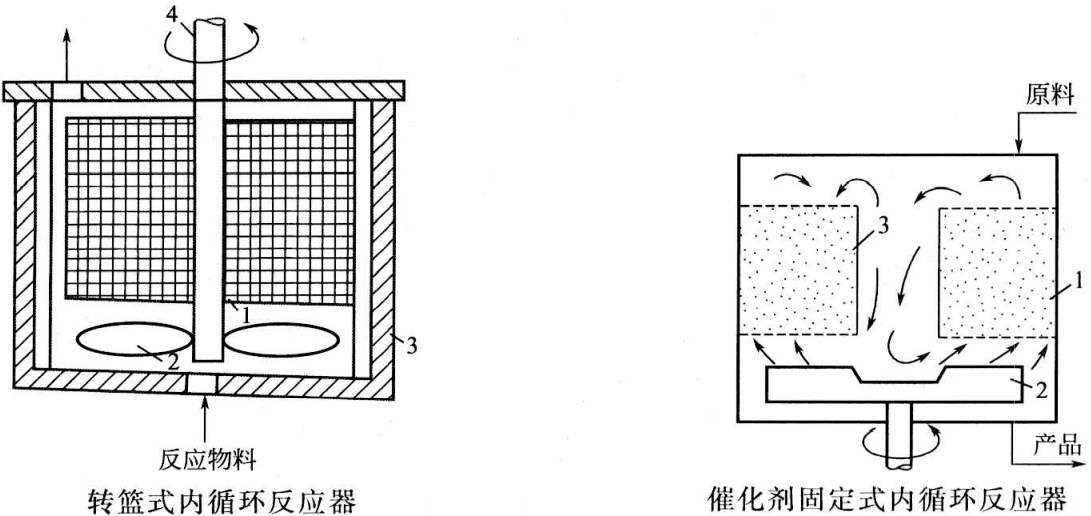
\includegraphics[width=.5\linewidth]{figures/fig7.15.png}
    \end{figure}

\end{frame}